\begin{frame}[standout]

{\huge \normalfont \sansc appendix}

\end{frame}

\begin{frame}[c]\frametitle{Gold Annotator Agreement}

\centering
\begin{tikzpicture}
  \begin{axis}[
      mbarplot,
      cycle list name=mbarplot cycle,
      width  = \columnwidth,
      height = 0.98\textheight,
      major x tick style = transparent,
      ybar=\pgflinewidth,
      bar width=15pt,
      ymajorgrids = true,
      ylabel = {Cohen's Kappa},
      symbolic x coords={r/AskParents, r/needadvice},
      xtick = data,
      tick label style={/pgf/number format/assume math mode=true},
      scaled y ticks = false,
      enlarge x limits=0.5,
      ymin=0,
      ymax=1,
      legend cell align=left,
      legend style={
              at={(0.9,0.99)},
              anchor=north,
              text=fgcolor,
             font=\normalsize
      }
  ]
   \addplot+
          coordinates {(r/AskParents, 0.620) (r/needadvice, 0.669)};
   \addplot+[style={postaction={pattern=crosshatch dots}}]
          coordinates {(r/AskParents, 0.680) (r/needadvice, 0.681)};
   \legend{$\kappa_{maj}$, $\kappa_{DS}$}
  \end{axis}
\end{tikzpicture}

\end{frame}

\begin{frame}[c]\frametitle{Average  Inter-Annotator Agreement}

\centering
\begin{tikzpicture}
  \begin{axis}[
      mbarplot,
      cycle list name=mbarplot cycle,
      width  = \columnwidth,
      height = 0.98\textheight,
      major x tick style = transparent,
      ybar=\pgflinewidth,
      bar width=15pt,
      ymajorgrids = true,
      ylabel = {Score},
      symbolic x coords={r/AskParents, r/needadvice},
      xtick = data,
      tick label style={/pgf/number format/assume math mode=true},
      scaled y ticks = false,
      enlarge x limits=0.5,
      ymin=0,
      ymax=100,
      legend cell align=left,
      legend style={
              at={(1.0,1.03)},
              anchor=north,
              text=fgcolor,
              font=\small
      }
  ]
  \addplot+
          coordinates {(r/AskParents, 83.71) (r/needadvice, 85.99)};
   \addplot+
          coordinates {(r/AskParents, 76.86) (r/needadvice, 85.71)};
   \addplot+
          coordinates {(r/AskParents, 79.62) (r/needadvice, 79.99)};
   \addplot+
          coordinates {(r/AskParents, 73.14) (r/needadvice, 79.55)};
   \legend{Accuracy, Precision, Recall, F1}
  \end{axis}
\end{tikzpicture}

\end{frame}

\begin{frame}[c]\frametitle{Lexical Analysis}

We quantify how strongly individual lemmas are associated with advice versus non-advice text using the log-odds ratio \citep{nye-nenkova-2015-identification}.

\vspace{5mm}

\begin{equation}
Odds(w,c) = \frac{P(w|c)}{1-P(w|c)}
\end{equation}

\begin{equation}
\text{log-odds ratio} = \frac{Odds(w,advice)}{Odds(w,non-advice))}
\end{equation}

\end{frame}

\begin{frame}[c]\frametitle{Generalizability Results}
\centering
\begin{tikzpicture}
  \begin{axis}[
      mbarplot,
      cycle list name=mbarplot cycle,
      width  = \columnwidth,
      height = 0.98\textheight,
      major x tick style = transparent,
      ybar=\pgflinewidth,
      bar width=15pt,
      ymajorgrids = true,
      ylabel = {F1},
      ylabel style={rotate=-90},
      symbolic x coords={r/AskParents, r/needadvice},
      xtick = data,
      tick label style={/pgf/number format/assume math mode=true},
      scaled y ticks = false,
      enlarge x limits=0.5,
      ymin=0,
      ymax=100,
      legend cell align=left,
      legend style={
              at={(0.9,0.99)},
              anchor=north,
              text=fgcolor,
              font=\small
      }
  ]
  \addplot+
          coordinates {(r/AskParents, 50.5) (r/needadvice, 77.8)};
   \addplot+[style={postaction={pattern=crosshatch dots}}]
          coordinates {(r/AskParents, 48.1) (r/needadvice, 76.0)};
   \legend{{\sansc normal\hphantom{er}}, {\sansc transfer}}
  \end{axis}
\end{tikzpicture}
\end{frame}

\begin{frame}[c]\frametitle{Dataset Metrics}
    \begin{table}[H]
        \centering
        \begin{tabular}{llll}
	\toprule
    \textbf{Dataset} & \textbf{Train} & \textbf{Dev} & \textbf{Test} \\
    \midrule
    AskParents & 8701(.29) & 802(.33) & 1091(.26)\\
    \midrule
    needadvice & 6148(.37) & 816(.34) & 898(.37) \\
    \bottomrule
\end{tabular}

        \caption{Sentence metrics in our dataset, with fraction DS-labeled as advice.}
        \label{tab:dataset-metrics}
    \end{table}
\end{frame}

\begin{frame}[c]\frametitle{Gold Internal Agreement}
    \begin{table}[H]
        \centering
        \begin{tabular}{llll}
	\toprule
    \textbf{Dataset} & \textbf{Sentences} & $\kappa_{maj}$ & $\kappa_{DS}$  \\
    \midrule
    AskParents & 203 & 0.620 & 0.669 \\
    \midrule
    needadvice & 110 & 0.680 & 0.681 \\
    \bottomrule
\end{tabular}

        \caption{Gold annotator agreement on the internal task.}
        \label{tab:internal-agreement}
    \end{table}
\end{frame}

\begin{frame}[c]\frametitle{Agreement}
    \begin{table}[H]
        \centering
        \begin{tabular}{lllll}
	\toprule
    \textbf{Dataset} & \textbf{Acc} & \textbf{P} & \textbf{R} & \textbf{F1}\\
    \midrule
    AskParents & 83.71 & 76.86 & 79.62 & 73.14 \\
    \midrule
    needadvice & 85.99 & 85.71 & 79.99 & 79.55 \\
    \bottomrule
\end{tabular}


        \caption{Average inter-annotator agreement for all workers against DS labels}
        \label{tab:agreement}
    \end{table}
\end{frame}

\begin{frame}[c]\frametitle{Discourse Modes}
    \begin{table}[H]
        \centering
        \begin{tabular}{lll}
	\toprule
    \textbf{Subreddit} & \textbf{Other (\%)} & \textbf{Personal}\\
     &  & \textbf{Narrative (\%)}\\
    \midrule
    \textbf{r/AskParents} & 83.6 & 16.4\\
    \midrule
    \textbf{r/needadvice} & 93.67 & 6.33 \\
    \textbf{\quad-Career} & 100 & 0\\
    \textbf{\quad-Mental Health} & 81.82 & 18.18\\
    \textbf{\quad-Friendships} & 100 & 0\\
    \textbf{\quad-Education} & 95.4 & 4.6\\
    \textbf{\quad-Life Decisions} & 88.9 & 11.1\\
    \bottomrule
\end{tabular}

        \caption{Modes of discourse for advice sentences in each flair/subreddit}
        \label{tab:disc-modes}
    \end{table}
\end{frame}

\begin{frame}[c]\frametitle{Results-Classification}
    \begin{table}[H]
        \centering
        \begin{tabular}{cllll}
	\toprule
    & \textbf{Model} & \textbf{P} & \textbf{R} & \textbf{F1} \\
    \midrule
    {\multirow{6}{*}{\rotatebox{90}{\tiny r/AskParents}}} & SEMEVAL & 32.7 & 70.2 & 44.6 \\
    & NTUA-IS & 31.4 & 64.9 & 42.3 \\
    & BERT$_{\text{noft}}$ & 62.6 (1.2) & 14.9 (1.0) & 24.0 (1.4) \\
    & BERT$_{\text{sent}}$ & 54.9 (2.4) & 49.5 (4.4) & \textbf{51.9} (1.9) \\
    & BERT$_{\text{sent+c}}$ & 54.2 (2.1) & 49.9 (4.0) & 51.9 (2.2) \\
    & BERT$_{\text{sent+q}}$ & 61.0 (13.4) & 33.1 (11.9) & 37.4 (8.1) \\
   \midrule
   {\multirow{6}{*}{\rotatebox{90}{\tiny r/needadvice}}} & SEMEVAL & 44.5 & 80.3 & 57.2 \\
    & NTUA-IS & 43.0 & 70.9 & 53.5 \\
    & BERT$_{\text{noft}}$ & 82.9 (0.5) & 44.6 (1.4) & 58.0 (1.2) \\
    & BERT$_{\text{sent}}$ & 79.7 (3.8) & 76.3 (3.9) & \textbf{77.8} (0.3) \\
    & BERT$_{\text{sent+c}}$ & 80.4 (4.4) & 75.3 (4.4) & 77.6 (0.7) \\
    & BERT$_{\text{sent+q}}$ & 83.4 (4.8) & 64.7 (7.4) & 72.5 (3.5) \\
    \bottomrule
\end{tabular}
        \caption{Classification results on test set.}
        \label{tab:results-class}
    \end{table}
\end{frame}

\begin{frame}[c]\frametitle{Results-Generalization}
    \begin{table}[H]
        \centering
        \begin{tabular}{lccc}
	\toprule
    \textbf{Model} & \textbf{P} & \textbf{R} & \textbf{F1} \\
    \midrule
     AP $\to$ AP & 54.9 (2.4) & 49.5 (4.4) & 51.9 (1.9) \\
     AP$_{p}$ $\to$ AP & 59.1 (3.5) & 44.4 (4.1) & 50.5 (1.8) \\
     NA $\to$ AP & 61.9 (4.9) & 39.7 (3.5) & 48.1 (1.3) \\
    \midrule
     NA $\to$ NA & 79.7 (3.8) & 76.3 (3.9) & 77.8 (0.3) \\
     AP $\to$ NA & 74.0 (4.0) & 79.3 (2.9) & 76.5 (0.9) \\
     AP$_{p}$ $\to$ NA & 76.9 (3.8) & 75.5 (4.7) & 76.0 (1.1) \\
    \bottomrule
\end{tabular}
        \caption{Generalizbility results on test set.}
        \label{tab:results-gen}
    \end{table}
\end{frame}

\begin{frame}[c]\frametitle{Results-Flair}
    \begin{table}[H]
        \centering
        \begin{tabular}{llll}
	\toprule
    \textbf{Flair} & \textbf{P} & \textbf{R} & \textbf{F1} \\
    \midrule
    Friendships & 85.5 (5.7) & 93.8 (0.0) & 89.2 (2.9) \\
    Mental Health & 75.6 (3.5) & 74.7 (3.6) & 75.0 (0.6) \\
    Education & 86.8 (2.9) & 67.4 (6.2) & 75.7 (3.1) \\
    Career & 75.9 (5.1) & 78.0 (3.8) & 76.7 (1.3)\\
    Life Decisions & 82.4 (4.4) & 82.8 (3.5) & 82.4 (0.7) \\
    \bottomrule
\end{tabular}
        \caption{Flair results on test set.}
        \label{tab:results-flair}
    \end{table}
\end{frame}

\begin{frame}[c]\frametitle{Attention}
   \begin{figure}
       \centering
       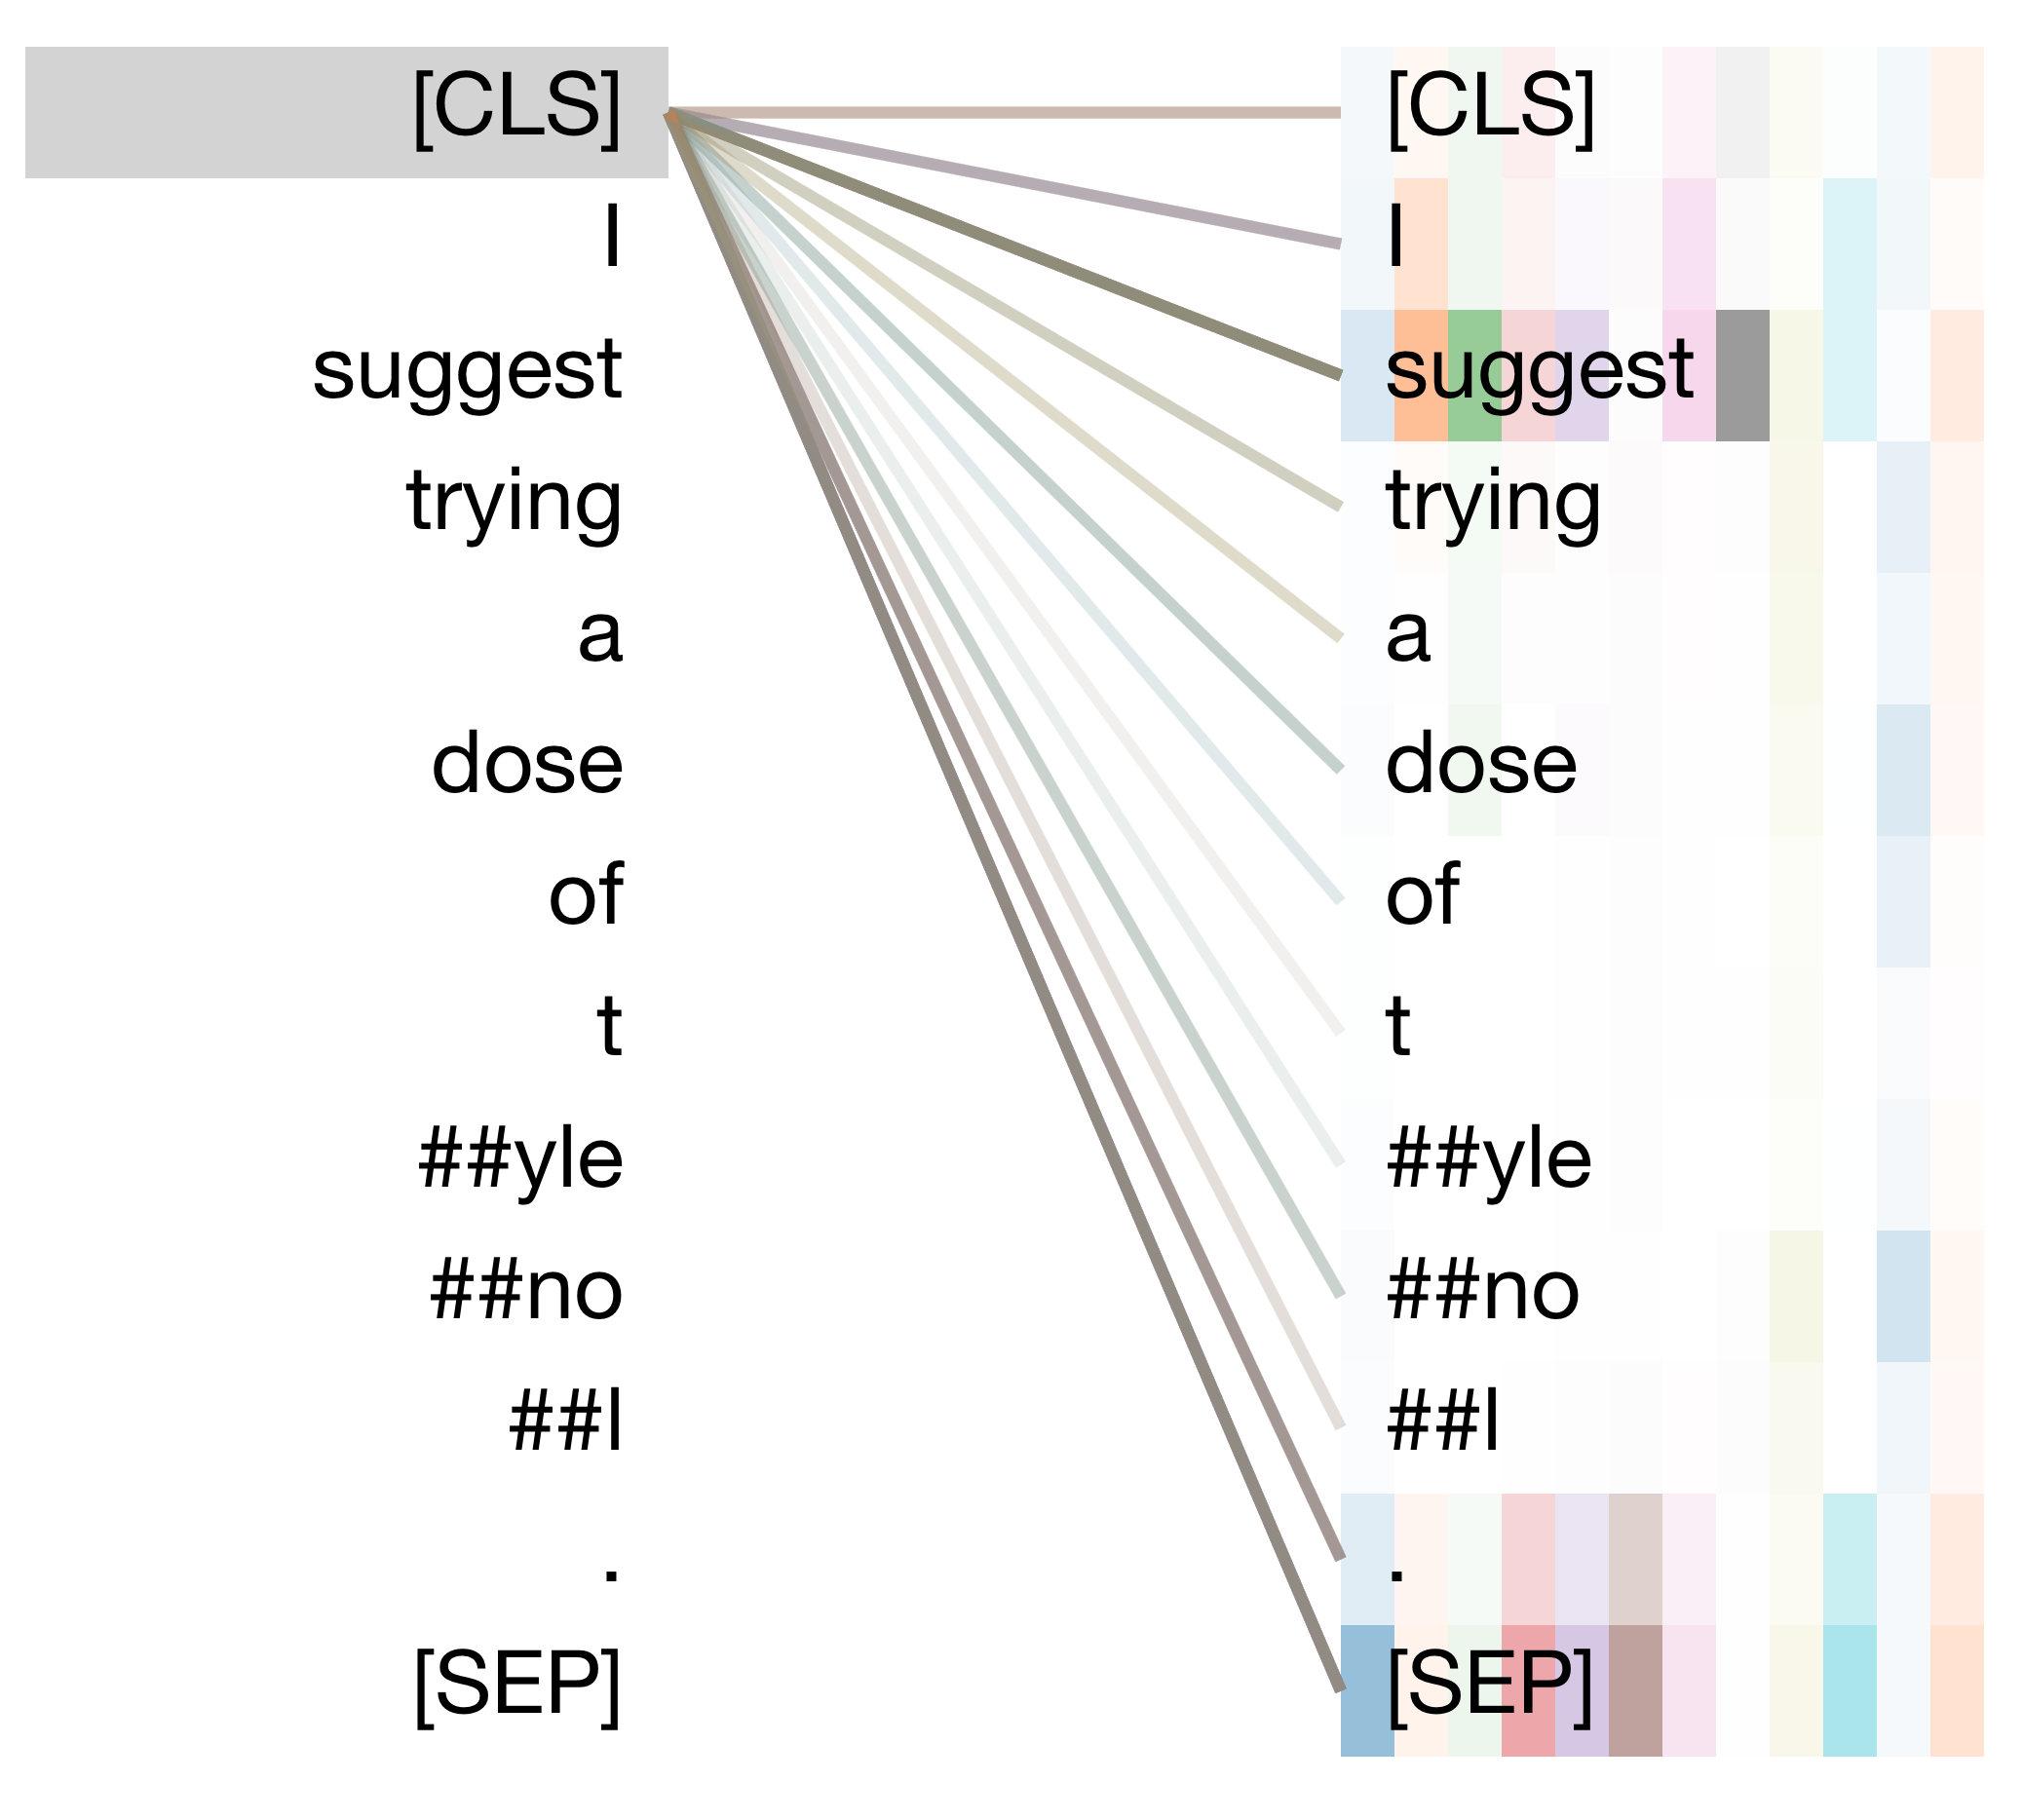
\includegraphics[width=0.75\linewidth]{figures/att-2.png}
       \caption{Attention weights visualized using BertViz~\citep{vig2019transformervis}}
   \end{figure}
\end{frame}

\begin{frame}[c]\frametitle{Attention}
    \begin{figure}
        \centering
        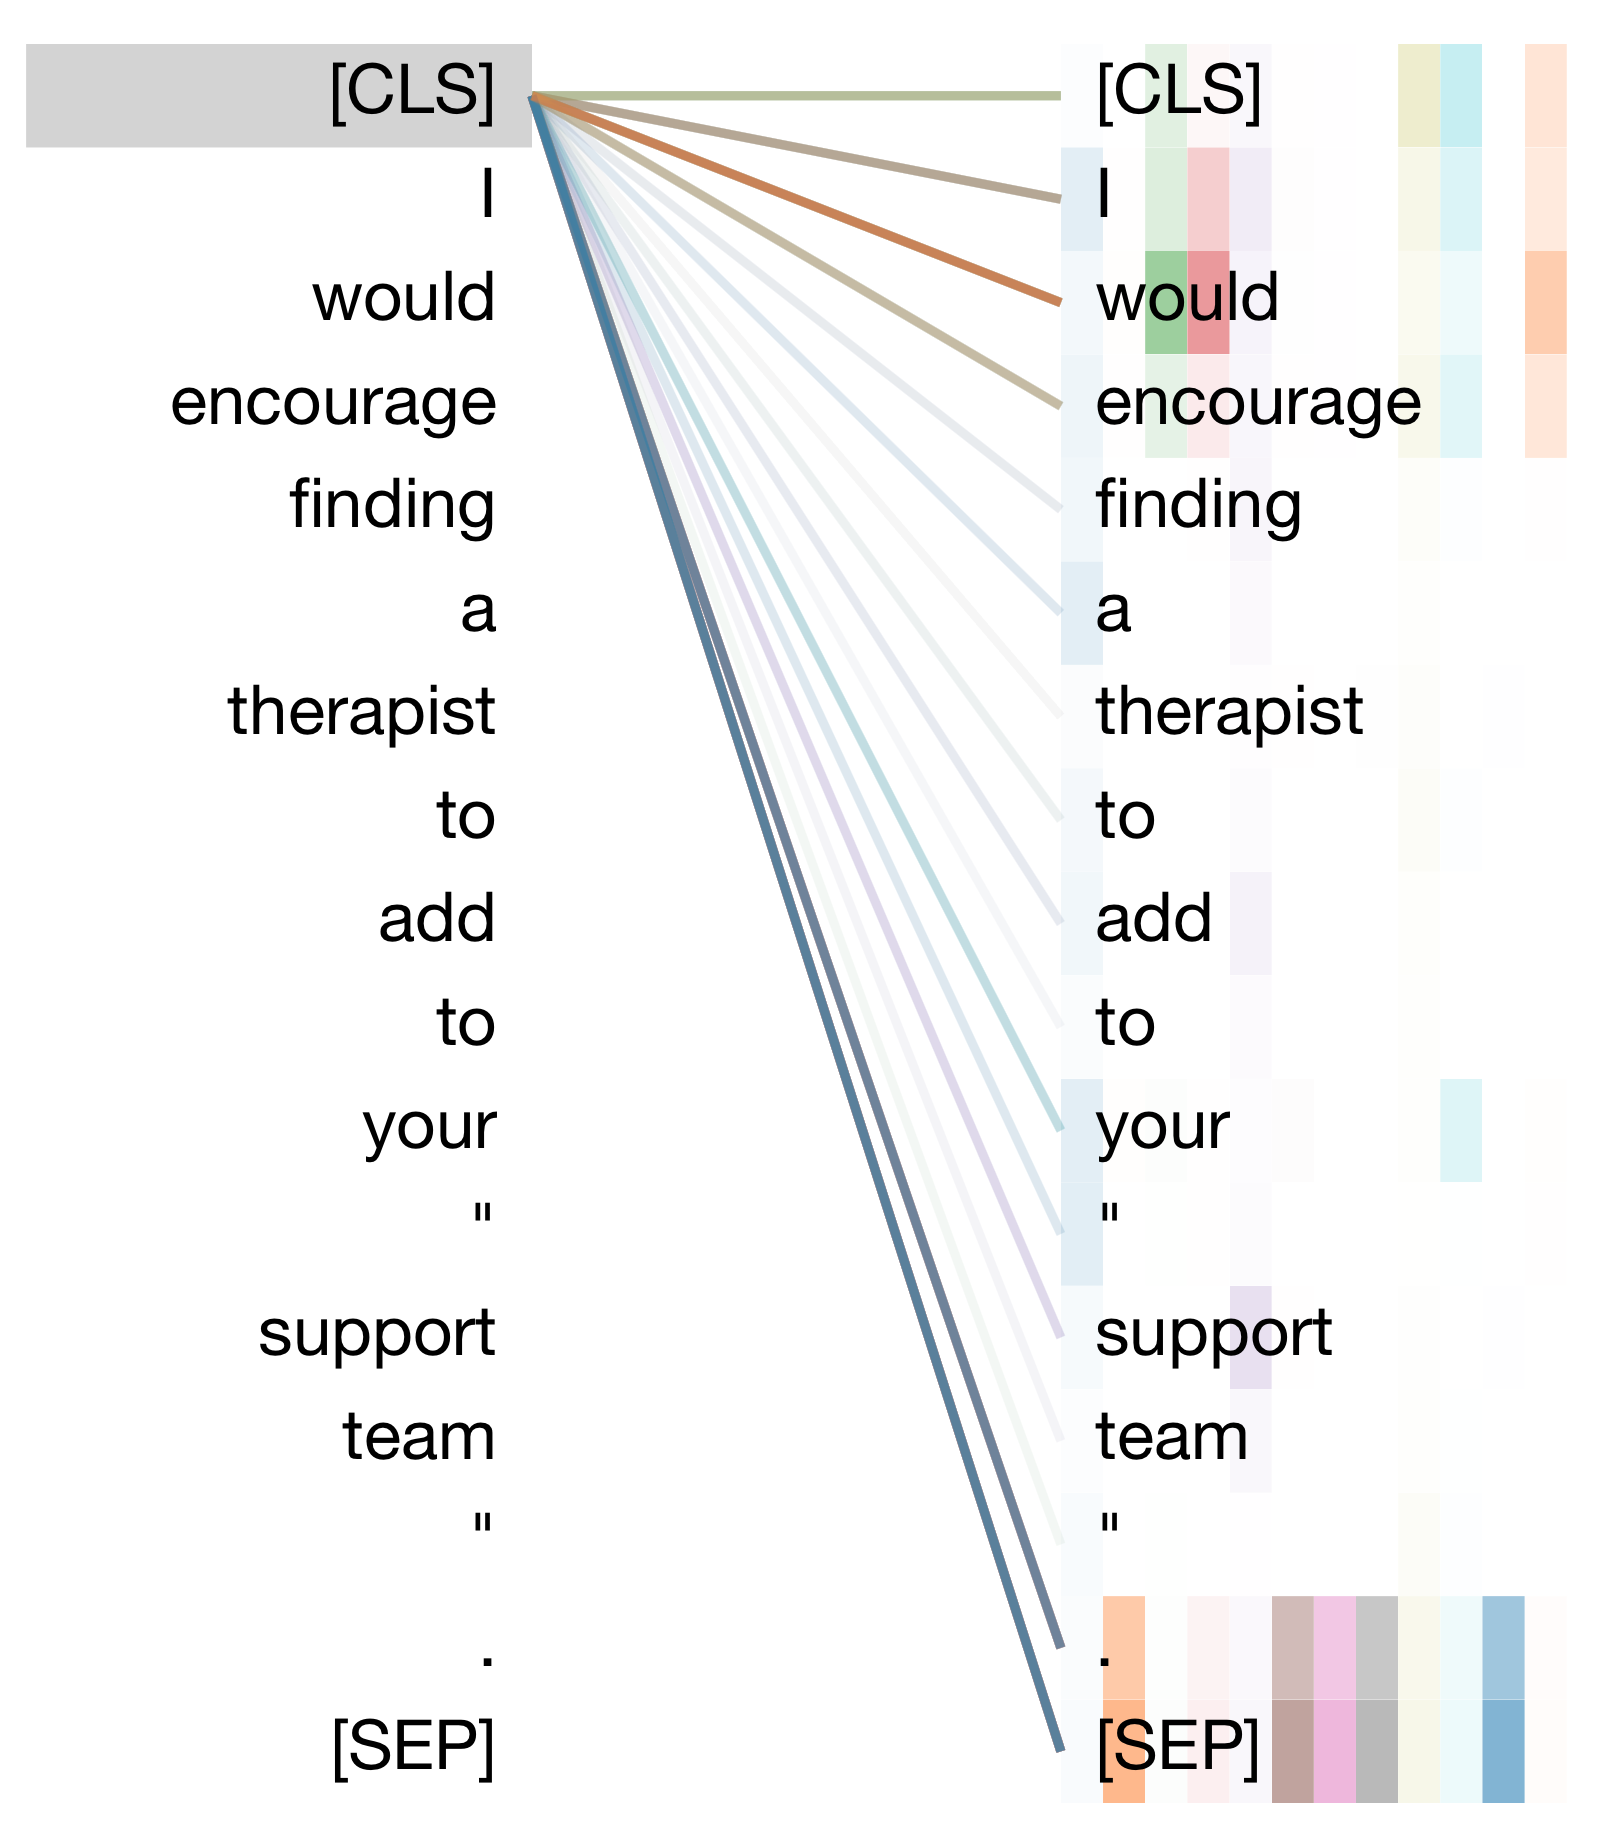
\includegraphics[width=0.6\linewidth]{figures/att-1.png}
        \caption{Attention weights visualized using BertViz~\citep{vig2019transformervis}}
    \end{figure}
\end{frame}